\section{Der Aufbau des Alten Testaments}\label{AufbauAT}
Jeder Vers des AT steht in einer eigenen Zeile, unabh�ngig, ob der Vers eher kurz ist, wie
"`Am Anfang schuf Gott Himmel und Erde."'

oder eher lang ist wie:
"`Da wurden berufen des K�nigs Schreiber zu der Zeit im dritten Monat, das ist der Monat Sivan, am dreiundzwanzigsten Tage, und wurde geschrieben, wie Mardochai gebot, an die Juden und an die F�rsten, Landpfleger und Hauptleute in den Landen von Indien bis an das Mohrenland, n�mlich hundert und siebenundzwanzig L�nder, einem jeglichen Lande nach seiner Schrift, einem jeglichen Volk nach seiner Sprache, und den Juden nach ihrer Schrift und Sprache."'

Die Zeilennummer identifiziert somit einen Vers eindeutig.

Neben den Versen gibt es auch noch Kapitel�berschriften wie z.B. "`Kapitel 1"' und Buchnamen wie z.B. "`1. Buch Mose"', die auch eine eindeutige Zeilennummer haben. Zur Vereinfachung wird auch bei Buchnamen und Kapiteln von Versen gesprochen. Die Verse eines Buches im AT sind zwar auch durchnummeriert, diese Nummerierung wird aber ignoriert, da sie nur innerhalb eines Kapitels eindeutig ist.
\begin{figure}[htp]
\centering
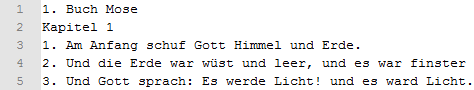
\includegraphics[width=1\textwidth]{Ingo/Bilder/AufbauAT.png}
\caption{Aufbau des AT}
\label{fig:AufbauAT}
\end{figure}